\chapter{Surrogate-Based Minimization}\label{sbm}

\section{Overview}\label{sbm:overview}

Surrogate models approximate an original, high fidelity ``truth''
model, typically at reduced computational cost.  In DAKOTA, several
surrogate model selections are possible, which are categorized as data
fits, multifidelity models, and reduced-order models, as described in
Section~\ref{models:surrogate}.  In the context of minimization
(optimization or calibration), surrogate models can speed convergence
by reducing function evaluation cost or smoothing noisy response
functions.

\section{Surrogate-Based Local Minimization}\label{sbm:sblm}

In the surrogate-based local minimization method (keyword:
\texttt{surrogate\_based\_local}) the minimization algorithm operates on
a surrogate model instead of directly operating on the computationally
expensive simulation model. The surrogate model can be based on data
fits, multifidelity models, or reduced-order models, as described in
Section~\ref{models:surrogate}. Since the surrogate will generally
have a limited range of accuracy, the surrogate-based local algorithm
periodically checks the accuracy of the surrogate model against the
original simulation model and adaptively manages the extent of the
approximate optimization cycles using a trust region approach.

%The surrogate-based local method in
%DAKOTA can be implemented using heuristic rules (less expensive) or
%provably-convergent rules (more expensive). The heuristic approach
%is particularly effective on real-world engineering design problems
%that contain nonsmooth features (e.g., slope discontinuities,
%numerical noise) where gradient-based optimization methods often have
%trouble, and where the computational expense of the simulation
%precludes the use of nongradient-based methods.

Refer to the DAKOTA Theory Manual~\cite{TheoMan} for algorithmic
details on iterate acceptance, merit function formulations,
convergence assessment, and constraint relaxation.


\subsection{SBO with Data Fits}\label{sbm:sblm:surface}

When performing SBO with local, multipoint, and global data fit
surrogates, it is necessary to regenerate or update the data fit for
each new trust region.  In the global data fit case, this can mean
performing a new design of experiments on the original high-fidelity
model for each trust region, which can effectively limit the approach
to use on problems with, at most, tens of variables.
Figure~\ref{fig:sbo_df} displays this case.  However, an important
benefit of the global sampling is that the global data fits can tame
poorly-behaved, nonsmooth, discontinuous response variations within
the original model into smooth, differentiable, easily navigated
surrogates.  This allows SBO with global data fits to extract the
relevant global design trends from noisy simulation data.

\begin{wrapfigure}{r}{.3\textwidth}
  \centering
  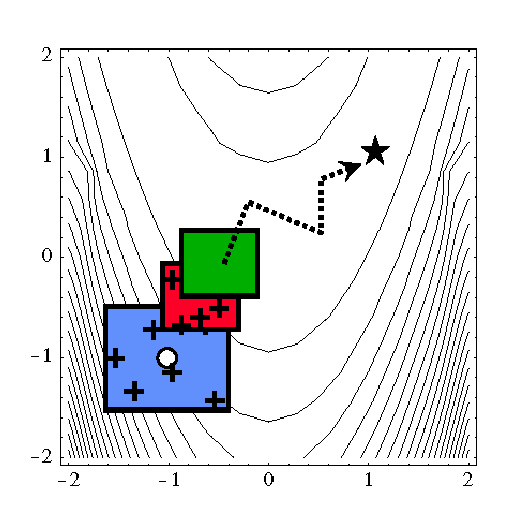
\includegraphics[width=.3\textwidth]{images/sbo_df}
  \caption{SBO iteration progression for global data fits.}
  \label{fig:sbo_df}
\end{wrapfigure}
When enforcing local consistency between a global data fit surrogate
and a high-fidelity model at a point, care must be taken to balance
this local consistency requirement with the global accuracy of the
surrogate.  In particular, performing a correction on an existing
global data fit in order to enforce local consistency can skew the
data fit and destroy its global accuracy.  One approach for achieving
this balance is to include the consistency requirement within the data
fit process by constraining the global data fit calculation (e.g.,
using constrained linear least squares).  This allows the data fit to
satisfy the consistency requirement while still addressing global
accuracy with its remaining degrees of freedom.
% Use figure from Theresa's paper?  Use equations from notes?
Embedding the consistency within the data fit also reduces the
sampling requirements.  For example, a quadratic polynomial normally
requires at least $(n+1)(n+2)/2$ samples for $n$ variables to perform
the fit.  However, with an embedded first-order consistency constraint
at a single point, the minimum number of samples is reduced by $n+1$ 
to $(n^2+n)/2$.
% With gradient information in each sample, this can be further
% reduced to ceil(n+2/2) samples.
%This corresponds to defining the terms of a symmetric Hessian matrix
%and points to an alternate approach.  Rather than enforcing
%consistency through constrained least squares, one can embed
%consistency directly by employing a Taylor series centered at the
%point of local consistency enforcement and globally estimating the
%higher order terms.  In the quadratic polynomial example, a
%second-order Taylor series with globally estimated Hessian terms
%requires the same $(n^2+n)/2$ samples and directly satisfies
%first-order consistency.  To further reduce sampling requirements in
%this case, one can choose to perform only partial updates (e.g., the
%diagonal) of the Hessian matrix~\cite{Per02}.

% Additional research area: Exploiting variance estimators to guide
% global search (e.g., kriging)

In the local and multipoint data fit cases, the iteration progression
will appear as in Fig.~\ref{fig:sbo_mh}.  Both cases involve a single
new evaluation of the original high-fidelity model per trust region,
with the distinction that multipoint approximations reuse information
from previous SBO iterates.  Like model hierarchy surrogates, these
techniques scale to larger numbers of design variables.  Unlike model
hierarchy surrogates, they generally do not require surrogate
corrections, since the matching conditions are embedded in the
surrogate form (as discussed for the global Taylor series approach
above).  The primary disadvantage to these surrogates is that the
region of accuracy tends to be smaller than for global data fits and
multifidelity surrogates, requiring more SBO cycles with smaller trust
regions.
%In SBO with surface fit functions, a sequence of optimization
%subproblems are evaluated, each of which is confined to a subset of
%the parameter space known as a ``trust region.'' Inside each trust
%region, DAKOTA's data sampling methods are used to evaluate the
%response quantities at a small number (order $10^{1}$ to $10^{2}$) of
%design points. Next, multidimensional surface fitting is performed to
%create a surrogate function for each of the response quantities.
%Finally, optimization is performed using the surrogate functions in
%lieu of the actual response quantities, and the optimizer's search is
%limited to the region inside the trust region bounds. A validation
%procedure is then applied to compare the predicted improvement in the
%response quantities to the actual improvement in the response
%quantities. Based on the results of this validation, the optimum
%design point is either accepted or rejected and the size of the trust
%region is either expanded, contracted, or left unchanged. The sequence
%of optimization subproblems continues until the SBO strategy
%convergence criteria are satisfied
More information on the design of experiments methods is available in
Chapter~\ref{dace}, and the data fit surrogates are described in
Section~\ref{models:surrogate:datafit}.

Figure~\ref{sbm:sblm_rosen} shows a DAKOTA input file that implements
surrogate-based optimization on Rosenbrock's function. This input file
is named \texttt{dakota\_sbo\_rosen.in} in the \texttt{Dakota/test}
directory.  The first method keyword block contains the SBO 
keyword \texttt{surrogate\_based\_local}, plus the commands for
specifying the trust region size and scaling factors. The optimization
portion of SBO, using the CONMIN Fletcher-Reeves conjugate gradient method,
is specified in the following keyword blocks for
\texttt{method}, \texttt{model}, \texttt{variables}, and
\texttt{responses}.  The model used by the optimization method 
specifies that a global surrogate will be used to map variables into
responses (no \texttt{interface} specification is used by the
surrogate model). The global surrogate is constructed using a DACE
method which is identified with the \texttt{`SAMPLING'} identifier.
This data sampling portion of SBO is specified in the final set of
keyword blocks for \texttt{method}, \texttt{model},
\texttt{interface}, and \texttt{responses} (the earlier 
\texttt{variables} specification is reused). This example problem uses 
the Latin hypercube sampling method in the LHS software to select 10
design points in each trust region. A single surrogate model is
constructed for the objective function using a quadratic polynomial.
The initial trust region is centered at the design point
$(x_1,x_2)=(-1.2,1.0)$, and extends $\pm 0.4$ (10\% of the global
bounds) from this point in the $x_1$ and $x_2$ coordinate directions.
\begin{figure}
  \begin{bigbox}
    \begin{tiny}
      \verbatimtabinput[8]{dakota_sbo_rosen.in}
    \end{tiny}
  \end{bigbox}
  \caption{DAKOTA input file for the surrogate-based local optimization
    example.}
  \label{sbm:sblm_rosen}
\end{figure}

If this input file is executed in DAKOTA, it will converge to the
optimal design point at $(x_{1},x_{2})=(1,1)$ in approximately 800
function evaluations. While this solution is correct, it is obtained
at a much higher cost than a traditional gradient-based optimizer
(e.g., see the results obtained from \texttt{dakota\_rosenbrock.in}).
This demonstrates that the SBO method with global data fits is not
really intended for use with smooth continuous optimization problems;
direct gradient-based optimization can be more efficient for such
applications. Rather, SBO with global data fits is best-suited for the
types of problems that occur in engineering design where the response
quantities may be discontinuous, nonsmooth, or may have multiple local
optima~\cite{Giu02}. In these types of engineering design problems,
traditional gradient-based optimizers often are ineffective, whereas
global data fits can extract the global trends of interest despite the
presence of local nonsmoothness (for an example problem with multiple
local optima, look in \texttt{Dakota/test} for the file
\texttt{dakota\_sbo\_sine\_fcn.in}~\cite{Giu00}).

The surrogate-based local minimizer is only mathematically
guaranteed to find a local minimum. However, in practice, SBO can often find 
the global minimum.  Due to the random sampling method used within the
SBO algorithm, the SBO method will solve a given problem a little differently 
each time it is run (unless the user specifies a particular random
number seed in the dakota input file as is shown in Figure~\ref{sbm:sblm_rosen}). 
Our experience on the quasi-sine function mentioned above is that if 
you run this problem 10 times with the same starting conditions but different 
seeds, then you will find the global minimum in about 70-80\% of the trials.
This is good performance for what is mathematically only a local optimization method.

\subsection{SBO with Multifidelity Models}\label{sbm:sblm:multifidelity}

When performing SBO with model hierarchies, the low-fidelity model is
normally fixed, requiring only a single high-fidelity evaluation to
compute a new correction for each new trust region.
Figure~\ref{fig:sbo_mh} displays this case.  This renders the
multifidelity SBO technique more scalable to larger numbers of design
variables since the number of high-fidelity evaluations per iteration
(assuming no finite differencing for derivatives) is independent of
the scale of the design problem.  However, the ability to smooth
poorly-behaved response variations in the high-fidelity model is lost,
and the technique becomes dependent on having a well-behaved
low-fidelity model\footnote{It is also possible to use a hybrid data
fit/multifidelity approach in which a smooth data fit of a noisy low
fidelity model is used in combination with a high fidelity model}.  In
addition, the parameterizations for the low and high-fidelity models
may differ, requiring the use of a mapping between these
parameterizations.  Space mapping, corrected space mapping, POD
mapping, and hybrid POD space mapping are being explored for this
purpose~\cite{Rob06a,Rob06b}.

\begin{wrapfigure}{r}{.3\textwidth}
  \centering
  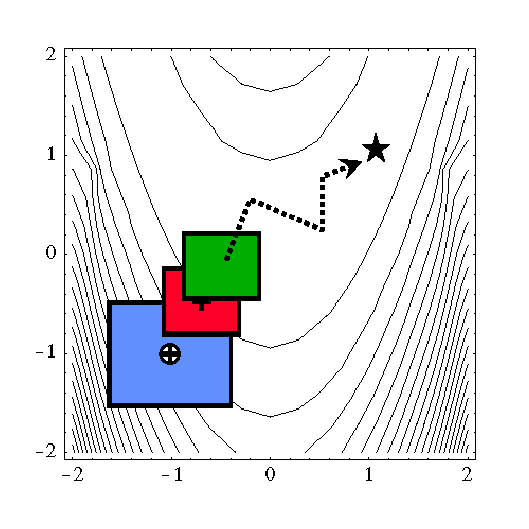
\includegraphics[width=.3\textwidth]{images/sbo_mh}
  \caption{SBO iteration progression for model hierarchies.}
  \label{fig:sbo_mh}
\end{wrapfigure}
%\begin{figure}
%\epsfxsize 3in
%\centerline{\epsfbox{sbo_mh.eps}}
%\caption{SBO iteration progression for model hierarchies.}
%\label{fig:sbo_mh}
%\end{figure}

When applying corrections to the low-fidelity model, there is no
concern for balancing global accuracy with the local consistency
requirements.  However, with only a single high-fidelity model evaluation
at the center of each trust region, it is critical to use the best
correction possible on the low-fidelity model in order to achieve
rapid convergence rates to the optimum of the high-fidelity
model~\cite{Eld04}.

%SBO can also be applied with multifidelity, or hierarchical, models,
%i.e., where one has available both a high-fidelity computational model
%and a low-fidelity computational model. This situation can occur when
%the low-fidelity model neglects some physical phenomena (e.g.,
%viscosity, heat transfer, etc.) that are included in the high-fidelity
%model, or when the low-fidelity model has a lower resolution
%computational mesh than the high-fidelity model. In many cases, the
%low-fidelity model can serve as a surrogate for the high-fidelity
%model during the optimization process. Thus, the low-fidelity model
%can be used in SBO in a manner similar to the use of surface fit
%models described in Section~\ref{sbm:sblm:surface}. A key difference
%in SBO with hierarchical surrogates is that a design of experiments
%using the high-fidelity model is not required; rather high-fidelity
%evaluations are only needed at the center of the current trust-region
%and the predicted optimum point in order to correct the low-fidelity
%model and verify improvement, respectively. Another difference is that
%one of the four types of correction described in
%Section~\ref{sbm:sblm:surface} is required for SBO with multifidelity
%models.

A multifidelity test problem named
\texttt{dakota\_sbo\_hierarchical.in} is available in
\texttt{Dakota/test} to demonstrate this SBO approach. This test
problem uses the Rosenbrock function as the high fidelity model and a
function named ``lf\_rosenbrock'' as the low fidelity model. Here,
lf\_rosenbrock is a variant of the Rosenbrock function (see
\texttt{Dakota/test/lf\_rosenbrock.C} for formulation) with the
minimum point at $(x_1,x_2)=(0.80,0.44)$, whereas the minimum of the
original Rosenbrock function is $(x_1,x_2)=(1,1)$. Multifidelity SBO
locates the high-fidelity minimum in 11 high fidelity evaluations for
additive second-order corrections and in 208 high fidelity evaluations
for additive first-order corrections, but fails for zeroth-order
additive corrections by converging to the low-fidelity minimum.

\subsection{SBO with Reduced Order Models}\label{sbm:sblm:rom}

When performing SBO with reduced-order models (ROMs), the ROM is
mathematically generated from the high-fidelity model.  A critical
issue in this ROM generation is the ability to capture the effect of
parametric changes within the ROM.  Two approaches to parametric ROM
are extended ROM (E-ROM) and spanning ROM (S-ROM)
techniques~\cite{Wei06}.  Closely related techniques include tensor
singular value decomposition (SVD) methods~\cite{Lat00}.  In the
single-point and multipoint E-ROM cases, the SBO iteration can appear
as in Fig.~\ref{fig:sbo_mh}, whereas in the S-ROM, global E-ROM, and
tensor SVD cases, the SBO iteration will appear as in
Fig.~\ref{fig:sbo_df}.  In addition to the high-fidelity model
analysis requirements, procedures for updating the system matrices and
basis vectors are also required.

Relative to data fits and multifidelity models, ROMs have some
attractive advantages.  Compared to data fits such as regression-based
polynomial models, they are more physics-based and would be expected
to be more predictive (e.g., in extrapolating away from the immediate
data).  Compared to multifidelity models, ROMS may be more practical
in that they do not require multiple computational models or meshes
which are not always available.  The primary disadvantage is potential
invasiveness to the simulation code for projecting the system using
the reduced basis.


\section{Surrogate-Based Global Minimization}\label{sbm:sbgm}

Surrogate-based global minimization differs from the surrogate-based 
local minimization approach discussed in the previous section in several ways: 
it is not a trust-region approach; initially there is one surrogate 
constructed over a set of sample points and the optimizer operates on that 
surrogate (as opposed to adaptively selecting points and re-building a 
surrogate in each trust region); and there is no guarantee of convergence. 

The \texttt{surrogate\_based\_global} method was developed to address
two needs.  The first is the case where a user wishes to use existing
function evaluations or a fixed sample size (perhaps based on
computational cost and allocation of resources) to build a surrogate
once and optimize on it.  In this case (a single global optimization
on a surrogate model), the set of surrogate building points is
determined in advance as opposed to the trust-region local surrogate
optimization in which the number of ``true'' function evaluations
depends on the location and size of the trust region, the goodness of
the surrogate within the trust-region, and problem characteristics.

In the second \texttt{surrogate\_based\_global} use case, we want to
update the surrogate, but globally.  That is, we add points to the
sample set used to create the surrogate, rebuild the surrogate, and
then perform another global optimization on the new surrogate.  Thus,
surrogate-based global optimization can be used in an iterative
scheme.  In one iteration, minimizers of the surrogate model are
found, and a selected subset of these are passed to the next
iteration.  In the next iteration, these surrogate points are
evaluated with the ``truth'' model, and then added to the set of
points upon which the next surrogate is constructed.  This presents a
more accurate surrogate to the minimizer at each subsequent iteration,
presumably driving to optimality quickly.  Note that a global
surrogate is constructed using the same bounds in each iteration.
This approach has no guarantee of convergence.

The surrogate-based global method was originally designed for MOGA (a
multi-objective genetic algorithm).  Since genetic algorithms often
need thousands or tens of thousands of points to produce optimal or
near-optimal solutions, surrogates can help by reducing the necessary
truth model evaluations.  Instead of creating one set of surrogates
for the individual objectives and running the optimization algorithm
on the surrogate once, the idea is to select points along the
(surrogate) Pareto frontier, which can be used to supplement the
existing points.  In this way, one does not need to use many points
initially to get a very accurate surrogate.  The surrogate becomes
more accurate as the iterations progress.

Most single objective optimization methods will return only a single
optimal point.  In that case, only one point from the surrogate model
will be evaluated with the ``true'' function and added to the pointset
upon which the surrogate is based.  In this case, it will take many
iterations of the surrogate-based global optimization for the approach
to converge, and its utility may not be as great as for the
multi-objective case when multiple optimal solutions are passed from
one iteration to the next to supplement the surrogate.  Note that the
user has the option of appending the optimal points from the surrogate
model to the current set of truth points or using the optimal points
from the surrogate model to replace the optimal set of points from the
previous iteration.  Although appending to the set is the default
behavior, at this time we strongly recommend using the option
\texttt{replace\_points} because it appears to be more accurate and
robust.

When using the surrogate-based global method, we first recommend
running one optimization on a single surrogate model. That is, set
\texttt{max\_iterations} to 1.  This will allow one to get a sense of
where the optima are located and also what surrogate types are the
most accurate to use for the problem.  Note that by fixing the seed of
the sample on which the surrogate is built, one can take a DAKOTA
input file, change the surrogate type, and re-run the problem without
any additional function evaluations by specifying the use of the
dakota restart file which will pick up the existing function
evaluations, create the new surrogate type, and run the optimization
on that new surrogate.  Also note that one can specify that surrogates
be built for all primary functions and constraints or for only a
subset of these functions and constraints.  This allows one to use a
"truth" model directly for some of the response functions, perhaps due
to them being much less expensive than other functions.  Finally, a
diagnostic threshold can be used to stop the method if the surrogate
is so poor that it is unlikely to provide useful points.  If the
goodness-of-fit has an R-squared value less than 0.5, meaning that
less than half the variance of the output can be explained or
accounted for by the surrogate model, the surrogate-based global
optimization stops and outputs an error message.  This is an arbitrary
threshold, but generally one would want to have an R-squared value as
close to 1.0 as possible, and an R-squared value below 0.5 indicates a
very poor fit.

For the surrogate-based global method, we initially recommend a small
number of maximum iterations, such as 3--5, to get a sense of how the
optimization is evolving as the surrogate gets updated globally.  If
it appears to be changing significantly, then a larger number (used in
combination with restart) may be needed.

Figure~\ref{sbm:sbgm_moga} shows a DAKOTA input file that implements
surrogate-based global optimization on a multi-objective test function. 
This input file
is named \texttt{dakota\_su\_mogatest1.in} in the \texttt{Dakota/test}
directory.  The first method keyword block contains the
keyword \texttt{surrogate\_based\_global}, plus the commands for
specifying five as the maximum iterations and the option to replace 
points in the global surrogate construction. The method block identified 
as MOGA specifies a multi-objective genetic algorithm optimizer and its 
controls.  The model keyword block specifies a surrogate model.  
In this case, a \texttt{gaussian\_process} model is used as a surrogate. 
The \texttt{dace\_method\_pointer} specifies that the surrogate will be 
build on 100 Latin Hypercube samples with a seed = 531.
The remainder of the input specification deals with the interface 
to the actual analysis driver and the 2 responses being returned 
as objective functions from that driver. 

\begin{figure}
  \begin{bigbox}
    \begin{tiny}
      \verbatimtabinput[8]{dakota_su_mogatest1.in}
    \end{tiny}
  \end{bigbox}
  \caption{DAKOTA input file for the surrogate-based global optimization
    example.}
  \label{sbm:sbgm_moga}
\end{figure}
 
\section{Efficient Global Minimization}\label{sbm:egm}

Efficient Global Optimization (EGO) is a global optimization technique
that employs response surface surrogates~\cite{Jon98,Hua06}.  In each
EGO iteration, a Gaussian process (GP) approximation for the objective
function is constructed based on sample points of the true simulation.
The GP allows one to specify the prediction at a new input location as
well as the uncertainty associated with that prediction.  The key idea
in EGO is to maximize an Expected Improvement Function (EIF), defined
as the expectation that any point in the search space will provide a
better solution than the current best solution, based on the expected
values and variances predicted by the GP model.  It is important to
understand how the use of this EIF leads to optimal solutions.  The
EIF indicates how much the objective function value at a new potential
location is expected to be less than the predicted value at the
current best solution.  Because the GP model provides a Gaussian
distribution at each predicted point, expectations can be calculated.
Points with good expected values and even a small variance will have a
significant expectation of producing a better solution (exploitation),
but so will points that have relatively poor expected values and
greater variance (exploration).  The EIF incorporates both the idea of
choosing points which minimize the objective and choosing points about
which there is large prediction uncertainty (e.g., there are few or no
samples in that area of the space, and thus the probability may be
high that a sample value is potentially lower than other values).
Because the uncertainty is higher in regions of the design space with
few observations, this provides a balance between exploiting areas of
the design space that predict good solutions, and exploring areas
where more information is needed.

There are two major differences between our implementation and that of
~\cite{Jon98}: we do not use a branch and bound method to find points
which maximize the EIF.  Rather, we use the DIRECT algorithm.  Second,
we allow for multiobjective optimization and nonlinear least squares
including general nonlinear constraints.  Constraints are handled
through an augmented Lagrangian merit function approach (see
Surrogate-Based Minimization chapter in DAKOTA Theory
Manual~\cite{TheoMan}).

The method is specified as \texttt{efficient\_global}.  Currently we
do not expose any specification controls for the underlying Gaussian
process model used or for the optimization of the expected improvement
function, which is currently performed by the NCSU DIRECT
algorithm. The only item the user can specify is a seed which is 
used in the Latin Hypercube Sampling to generate the initial 
set of points which is used to construct the initial Gaussian process. 
An example specification for the EGO algorithm is shown in
Figure~\ref{sbm:egm_rosen}.  This can be found in the 
\texttt{dakota\_rosenbrock\_ego.in} file in the 
\texttt{Dakota/test} directory.
\begin{figure}
  \begin{bigbox}
    \begin{small}
      \verbatimtabinput[8]{dakota_rosenbrock_ego.in}
    \end{small}
  \end{bigbox}
  \caption{DAKOTA input file for the efficient global optimization example.}
  \label{sbm:egm_rosen}
\end{figure}

